\setcounter{chapter}{5}
\chapter{Introduction to Packings}

\scribe{Ferran Dachs Cadefau}


For the first part see \cite{Pfeifle}.
\section{Big numbers}

Using computers, you can represent big numbers, you can do: 

\renewcommand{\arraystretch}{1.5}
\begin{tabular}{|c|c|c|}
\hline
$\NN$, $\ZZ$	 	&\texttt{int, long int, long long int} 			&$-9.2 \cdot 10^{18} ... 9.2 \cdot 10^{18}$	\\
			&or work with arbitrary precision (slower)		&\texttt{gmplib.org}				\\
\hline
$\QQ$			&$\{(n, d) : n \in \ZZ, d \in \NN_{>0} \}/\sim$		&\texttt{gmplib.org}				\\
			&where $(n, d) \sim (n' , d' )$ iff $nd' = n'd$		&						\\
\hline
$\RR$			&algebraic numbers ok ( $\sqrt{2}$, $\sqrt[4]{3}$),	&\texttt{cgal.org, mpfr.org}			\\
			&transcendental ones not ($\pi$, e)			&						\\
\hline
$\CC$, $\HH$		&pairs or quadruples of reals				&\texttt{\#include <complex>}			\\
\hline
\end{tabular}


But how to represent a very big numbers? For example using 4 symbols what is the biggest number that you can represent?

$$10^{99} < 9^{999} < 9^{9^{9^9}} = 9 \uparrow 4 < 9 \uparrow 9 \uparrow 9 \uparrow 9 = 9 \uparrow \uparrow 4 < 9 \Uparrow 9 \Uparrow 9 \Uparrow 9$$

This is known as Knuth's up-arrow notation, to represent bigger numbers there are the Ackerman Function:

$$A(k,n) = n \Uparrow^{(k)} n$$
$$A(n,n) = n \Uparrow^{(n)} n$$

For example:

$$A(2)= 2 \Uparrow 2 = 2 \uparrow 2 \uparrow 2 = 2 \uparrow \left( 2^2\right) = 2^{2^{2^2}}$$
$$A(3)= 3 \Uparrow^{(3)} 3 = 3 \Uparrow 3 \Uparrow 3 \Uparrow 3$$

Using this we can define $\alpha(x)$ as:

$$\alpha(x)=\max\{n\in\NN_{\geqslant 1}:A(n)<x\}$$

It appears, for example, in the complexity of the lower envelope of a segment arrangement. In the plane is $\Omega(n\alpha(n))$

\section{Projective geometry and Polarity}
\subsection{Projective geometry}

We define the projective space as:

$$\begin{array}{rcl}
   \Proj^n	&=	&\{\text{lines through }0\in\RR^{n+1} \}	\\
		&=	&S^n/\ZZ_2
  \end{array}
$$

We are identifying the antipodes: $x$ and $-x$. But we have a problem: $\Proj^1$, $\Proj^3$ are orientable, but for example $\Proj^2$ not: we can't define interior (inside/outside), therefore we can't define convex.

In $\Proj^2$ The line through points $p_1$ and $p_2$:

\begin{itemize}
\item $p_1$ lies on $l$: $p_1\perp l$
\item $p_2$ lies on $l$: $p_2\perp l$
\end{itemize}

Therefore: $l = \lambda \cdot  p_1 \times p_2$ ($\times$ is the cross-product of vectors in $\RR^3$, in higher dimensions is the determinant).

The point $q$ on lines $l_1$ and $l_2$:

\begin{itemize}
\item $q$ lies on $l_1$: $q\perp l_1$
\item$q$ lies on $l_2$: $q\perp l_2$
\end{itemize}

Therefore: $q = \lambda \cdot l_1 \times l_2$ (the cross-product of vectors in $\RR^3$, in higher dimensions is the determinant).

Computationally, we can intersect lines and join points, in homogeneous coordinates or in Cartesian coordinates. In the first case we have:

\texttt{void intersect\_lines(const vec\_t\& l1, const vec\_t\& l2, vec\_t\& p)}

\texttt{\{}

\texttt{cross\_product(l1, l2, p);}

\texttt{\}}

\texttt{void join\_points(const vec\_t\& p1, const vec\_t\& p2, vec\_t\& l)}

\texttt{\{}

\texttt{cross\_product(p1, p2, l);}

\texttt{\}}

\texttt{void cross\_product(const vec\_t\& l1, const vec\_t\& l2, vec\_t\& p)}

\texttt{\{}

\texttt{p[0] = l1[1]*l2[2] - l1[2]*l2[1];}

\texttt{p[1] = -l1[0]*l2[2] + l1[2]*l2[0];}

\texttt{p[2] = l1[0]*l2[1] - l1[1]*l2[0];}

\texttt{\}}

This code is \textbf{correct} (calculates exactly what it should), \textbf{efficient} (No extraneous copying (\&) and reuse of code), and \textbf{robust} (No influence of rounding errors and it handles all cases, even degenerate ones).


But, in Cartesian coordinates. A line is now $y = kx + d$, stored as a vector $(k , d)$.

\texttt{bool intersect\_lines(const vec\_t\& l1, const vec\_t\& l2, vec\_t\& p)}

\texttt{ \{}

\texttt{if (l1[0]==l2[0]) \{}

\texttt{if (l1[1]==l2[1]) \{}

\texttt{return COINCIDENT\_LINES;}

\texttt{\}}

\texttt{return PARALLEL\_LINES;}

\texttt{\}}

\texttt{p[0] = (l2[1]-l1[1])/(l1[0]-l2[0]);}

\texttt{p[1] = l1[0]*p[0] + l1[1];}

\texttt{\}}

This code is \textit{somewhat} \textbf{efficient} (Again, no copying, but: no reuse of code for join\_points), \textbf{not robust} (It's unstable numerically (==, /)), and \textit{not even} \textbf{correct} (It doesn't handle parallel lines, but that's Euclidean geometry's fault).


\subsection{Polarity}

It's related to \underline{Projective duality}, points are dual to hyperplanes:

$$\begin{array}{rcl}
    \Proj^n(\RR)	&\stackrel{d}{\longrightarrow}	&\left(\Proj^n(\RR)\right)^{\star}\\
    p			&\longmapsto				&p^{\star}
  \end{array}$$

A duality is an involutory order-antiisomorphism(Involution: $d^2=\id$, isomorphism: bijection collineation, order-anti: $p\in l$ implies $p\supset l$).

The polarity is the same except by convexs.

Polarity send: points to half-spaces. Given $a\in \RR^n$:

$$a\mapsto H_a=\{x\in\RR^d:\langle a,x\rangle\leqslant 1\}\leftrightarrow x\supset (\RR^d)^{\star}$$

Equivalently, they identify points with hyperplanes via homogeneous coordinates.

For example, if we take $p=(a:b:1)\in \overrightarrow{\Proj^2}$ a point, then $p^{\star}=(a:b:1)\in \left(\overrightarrow{\Proj^2}\right)^{\star}$ a line, and $p^{\star\star}=p$.

$P\in l\Leftrightarrow p\perp l\Leftrightarrow p^{\star}\perp l^{\star}\Leftrightarrow l^{\star}\perp p^{\star}\Leftrightarrow l^{\star}\in p^{\star}$ 

\section{Polymake}

Polymake is a free program in pearl. For example we can define a cube in dimension 3 as:

\texttt{polytope > \$p=cube(3);}

Another thing is know proprieties about a polytope. For example the coordinates of the vertices:

\texttt{polytope > print \$p->VERTICES;}

\texttt{1 -1 -1 -1}

\texttt{1 1 -1 -1}

\texttt{1 -1 1 -1}

\texttt{1 1 1 -1}

\texttt{1 -1 -1 1}

\texttt{1 1 -1 1}

\texttt{1 -1 1 1}

\texttt{1 1 1 1}

Or the number of faces of each dimension:

\texttt{polytope > print \$p->F\_VECTOR;}

\texttt{8 12 6}

Or the vertices in each facet:

\texttt{polytope > print \$p->VERTICES\_IN\_FACETS;}

\texttt{\{0 2 4 6\}}

\texttt{\{1 3 5 7\}}

\texttt{\{0 1 4 5\}}

\texttt{\{2 3 6 7\}}

\texttt{\{0 1 2 3\}}

\texttt{\{4 5 6 7\}}

To see a representation of the polytope you can execute:

\texttt{polytope > \$p-> VISUAL;}

\begin{figure}[htbp]
  \centering
  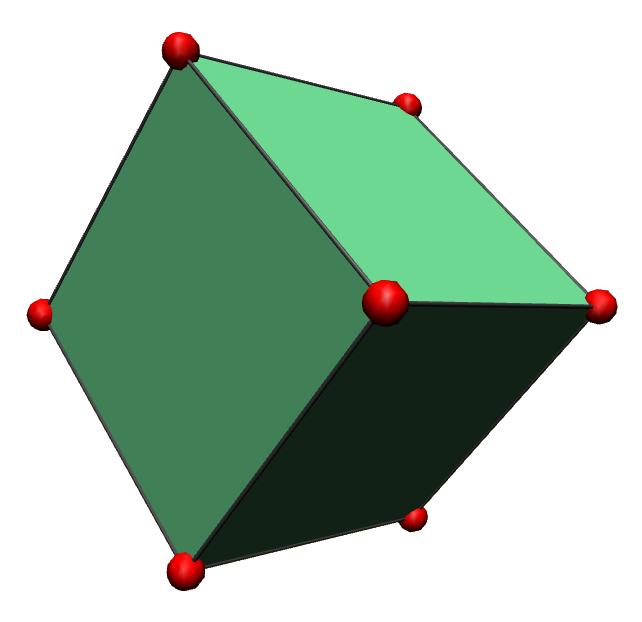
\includegraphics[width=.5\linewidth]{l6_cube.png}
  
  \caption{The representation of the cube in dimension 3 due with Polymake}
\label{fig:l6:1}
\end{figure}

To see a representation of graph of the polytope you can execute:

\texttt{polytope > \$p-> VISUAL\_FACE\_LATTICE;}

\begin{figure}[htbp]
  \centering
  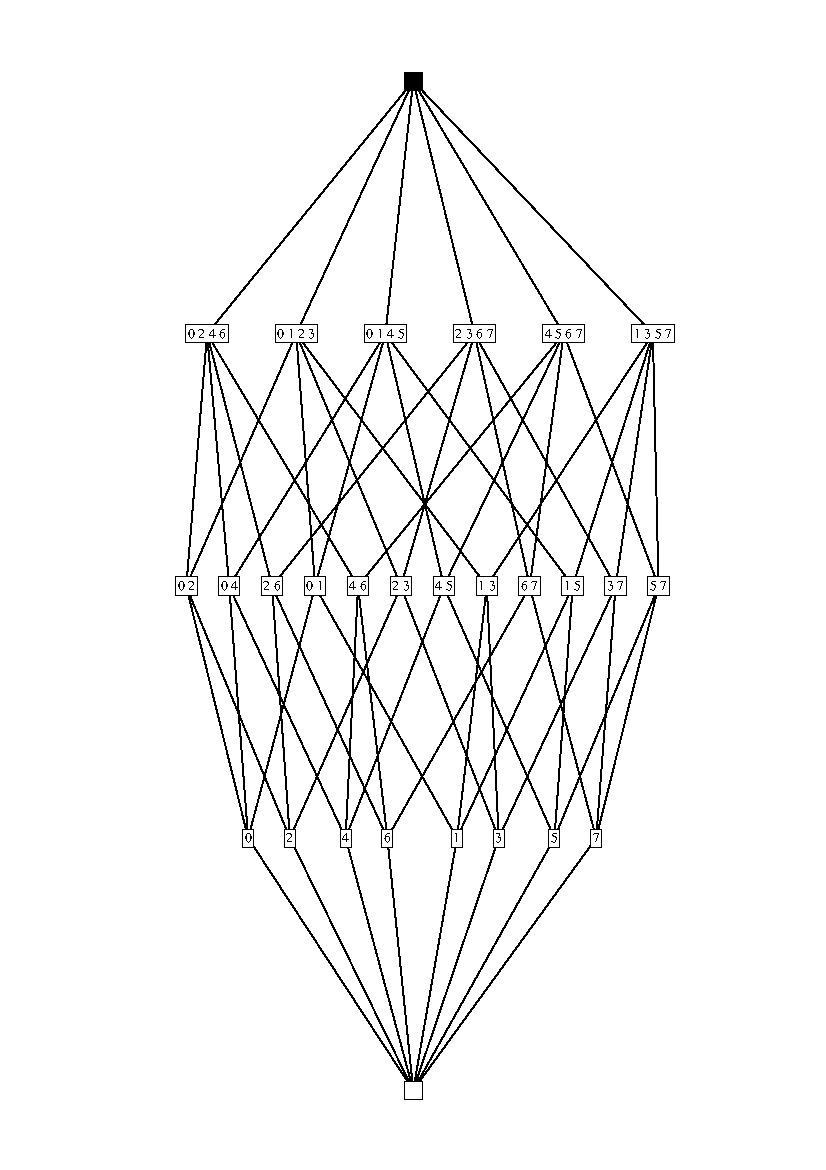
\includegraphics[width=0.9\linewidth]{l6_graph.jpg}
  
  \caption{The representation of the graph of the cube due with Polymake.}
\label{fig:l6:2}
\end{figure}

To see the equations of the facets you can type:

\texttt{polytope > print \$p->FACETS;}

\texttt{1 1 0 0}

\texttt{1 -1 0 0}

\texttt{1 0 1 0}

\texttt{1 0 -1 0}

\texttt{1 0 0 1}

\texttt{1 0 0 -1}

You must interpret as the following:

If you take $(1:1:0:0)$ gives you the facet: 

$$\left\langle(1:1:0:0)\left(\begin{array}{c}
                                                                     1\\	x\\	y\\	z
\end{array}\right)\right\rangle\geqslant 0$$

equivalently: $1+x\geqslant 0$ or $x\geqslant -1$. If you take $(1:-1:0:0)$ gives you the facet: $1-x\geqslant 0$ or $1\geqslant x$.
\newpage
We can polarize a polytope, for example:

\texttt{polytope > \$q=polarize(\$p);}

doing this, if we want to print the vertices of this new polytope, as we expected, gives the facets of the cube:

\texttt{polytope > print \$q->VERTICES;}

\texttt{1 -1 0 0}

\texttt{1 1 0 0}

\texttt{1 0 -1 0}

\texttt{1 0 1 0}

\texttt{1 0 0 -1}

\texttt{1 0 0 1}

Another thing that we can do is make Voronoi Diagrams. For example if we want to know the Voronoi Diagram of the points $(1,1),(0,1),(-1,1),(1,-1),(0,-1)\text{ and }(-1,-1)$:

\texttt{\$VD = new VoronoiDiagram(SITES=>[[1,1,1],[1,0,1],[1,-1,1],}

\texttt{[1,1,-1],[1,0,-1],[1,-1,-1]]);}

If we want to see a graphical representation:

\texttt{\$VD->VISUAL\_VORONOI;}

\begin{figure}[htbp]
  \centering
  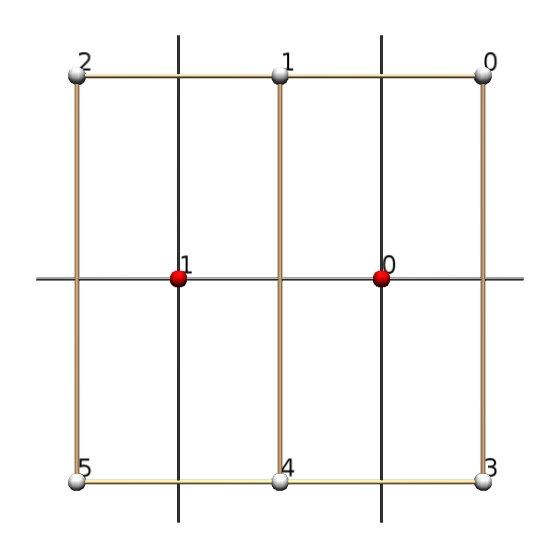
\includegraphics[width=0.7\linewidth]{l6_Voronoi.jpg}
  
  \caption{The representation of one Voronoi Diagram with Polymake.}
\label{fig:l6:3}
\end{figure}
\newpage
Other properties are, for example the facets equation:

\texttt{polytope > print \$VD->FACETS;}

\texttt{2 -2 -2 1}

\texttt{1 0 -2 1}

\texttt{2 2 -2 1}

\texttt{2 -2 2 1}

\texttt{1 0 2 1}

\texttt{2 2 2 1}

\texttt{1 0 0 0}

or the vertices of the diagram:

\texttt{polytope > print \$VD->VERTICES;}

\texttt{0 0 1 2}

\texttt{0 1 0 2}

\texttt{1 1/2 0 -1}

\texttt{0 -1 0 2}

\texttt{0 0 -1 2}

\texttt{1 -1/2 0 -1}

\section{Voronoi Cells in lattices}

Given a lattice $L\subset\RR^d$, find the facets of $$\Vor(0)=\{x\in\RR^d:\|x-0\|^2\leqslant\|x-v\|^2,\forall v\in L\}$$ 

\begin{defn}
 $v\in L$ is \textit{relevant} if the bisector of $v$ and $0$ contains a full dimensional face (i.e. a facet) of $\Vor(0)$.
\end{defn}

In $\ZZ^3$ we have a cube and the polytope defined by the relevant points is an octahedron.

\begin{obs}
 If the relevant vectors are precisely the minimal vector then $\Vor(0)$ is polar dual to the vertex figure of $0$ in $L$.
\end{obs}

\begin{theorem}[Georges Voronoi, 1908]
 A non-zero vector $v\in L$ is relevant if and only if $\pm v$ are the only shortest vectors in the coset $v+2L$.
\end{theorem}

\begin{proof}
 \underline{$\Longrightarrow$}

Suppose that $v,w\in L$ satisfy 

\begin{equation}\label{l6:eq1}
w\in v+2L 
\end{equation}

but

\begin{equation}\label{l6:eq2}
 w\neq \pm v
\end{equation}

and

\begin{equation}\label{l6:eq3}
 \langle w,w\rangle\leqslant \langle v,v\rangle
\end{equation}

Set:

\begin{center}
 $t=\frac{1}{2}(v+w)$ and  $u=\frac{1}{2}(v-w)$
\end{center}

Using (\ref{l6:eq1}) we have that $t,u\neq 0$ and using (\ref{l6:eq2}), $t,u\in L$. We have:

$$H_v=\{x\in\RR^d:\langle x,v\rangle\leqslant \frac{1}{2}\langle v,v\rangle\}$$

Let $x\in H_t\cap H_u$. Then:

$$\langle x,t\rangle\leqslant \frac{1}{2}\langle t,t\rangle$$ 

and

$$\langle x,u\rangle\leqslant \frac{1}{2}\langle u,u\rangle$$

Adding, we have:

$$\begin{array}{rcl}
   \langle x,v\rangle	&\leqslant	&\frac{1}{8}\left(\langle v,v\rangle+\langle w,w\rangle+2\langle v,w\rangle+\langle 							v,v\rangle+\langle w,w\rangle-\langle v,w\rangle\right)\\
			&=		&\frac{1}{4}\left(\langle v,v\rangle+\langle w,w\rangle\right)\\
			&\leqslant	&\frac{1}{2}\langle v,v\rangle
  \end{array}
$$ 

Were in the last one we have used (\ref{l6:eq3}). So $x\in H_v$, therefore $v$ is not relevant.

 \underline{$\Longleftarrow$}
Suppose $v\in L$ is not relevant. Then there exists some $w \in L$. $w\neq 0$, $w\neq \pm v$ with:

\begin{equation}\label{l6:eq4}
 \left\langle \frac{1}{2} v, w\right\rangle \geqslant \frac{1}{2}\langle w,w\rangle
\end{equation}

and $\frac{1}{2}v\notin H_w$.Then

$$\begin{array}{rcl}
   \|v-2w\|^2 	&=		&\langle v-2w,v-2w\rangle \\
		&=		&\langle v,v\rangle - 4 \langle v,w\rangle + 4 \langle w,w\rangle\\
		&\leqslant	&\langle v,v\rangle - 4 \langle v,w\rangle + 4 \langle v,w\rangle\\
		&=		&\langle v,v\rangle
  \end{array}
$$

where in the inequality we have used (\ref{l6:eq4}), and is in $v+2L$, not $0$, $w\in L$.

\end{proof}



